%%%%%%%%%%%%%%%%%%%%%%%%%%%%%%%%%%%%%%%%%%%%%%%%
\section{Module-Based Domain Behavior Language}
\label{sect:agl} 
%%%%%%%%%%%%%%%%%%%%%%%%%%%%%%%%%%%%%%%%%%%%%%%%

%The unified model is linked to an activity graph, which models the generic graph structure that is common to all activities. This activity graph incorporates module action to specialize the behavior of its nodes. In the terminology of the DDD's layer architecture~\cite{evans_domain-driven_2004}, the activity graph is positioned at the application layer, because it coordinates the behaviors of the modules owning the domain classes in the unified model in order to perform the overall activity's behavior.

%Figure~\ref{fig:agl-abstractSyntax} shows that ASM consists in \clazz{ModuleAct} (positioned at the top of the figure) and the UML activity graph, scoped by the inclusion, exclusion and restriction clauses in Section~\ref{sect:agl-abstractSyntax}. 
%From the language engineering perspective, we argue that the same benefits that are gained in unified domain modeling with \dcsl~can be attained for activity graphs if we develop a horizontal aDSL for them. We call this aDSL \abbrv{activity graph language}{\agl}. The language is used to create activity graphs by \textit{configuring} them directly on the domain model using annotations. We call a model that conforms to \agl~an \abbrv{activity graph configuration}{AGC}.

This section briefly specifies AGL as an aDSL for incorporating domain behaviors into a domain model. The language is used to create activity graphs by configuring them directly on the domain model using annotations. Adapting the meta-modeling approach for DSLs~\cite{kleppe_software_2008}, we focus on defining an \textit{abstract syntax meta-model} (ASM) and an annotation-based textual \textit{concrete syntax model (CSM)} for \agl. We only explain the syntactic aspects of \agl~since its behavioral semantics is characterized in Sections~\ref{sect:actSemantics} and~\ref{sect:behaviorPatterns}.
%
%More specifically, we construct the ASM in three steps. In the first step, we construct a conceptual model (CM) of the domain as a UML/OCL class diagram. This model helps understand the overall structure, without being constrained by the target OOPL's meta-model. The next two steps gradually transform CM into the ASM. In the second step, we transform CM into an equivalent, annotation-friendly form, called CM$_T$. In order to reduce the size of the eventual ASM, we try, in this step, to produce a compact CM$_T$. In the third step, we then transform CM$_T$ into the actual ASM, which takes an annotation-based form specified by the OOPL's meta-model. In this form, the configuration-related meta-concepts are represented by annotations. Further, we use Class as the basis to structure the annotations. 
%%%%%%%%%%%%%%%%%%%%%%%%%%%%%%%%%%%%%%%%%%%%%%%%%%%
\subsection{Abstract Syntax} 
\label{subsect:agl-abstractSyntax}
%%%%%%%%%%%%%%%%%%%%%%%%%%%%%%%%%%%%%%%%%%%%%%%%%%%

We describe the \agl's domain requirements in terms of the following inclusion (I), exclusion (X) and restriction (R) clauses that are applied to the UML activity graph requirements~\cite{omg_unified_2017}: (I1)~a module action (described in Section~\ref{sect:actSemantics}) as a special form of action~\cite[p.~442]{omg_unified_2017}; (R1)~an executable node~\cite[p.~403]{omg_unified_2017} performs a sequence of module actions; (R2)~a value specification~\cite[p.~374]{omg_unified_2017}) is only applied to decision nodes; (X1)~using a variable with activity (~\cite[p.~417]{omg_unified_2017}); (X2)~variable action~\cite[p.~467]{omg_unified_2017}; (X3)~an activity edge~\cite[p.~373]{omg_unified_2017} is without guards.

I1 and R1 are needed to incorporate the activity graph into MOSA. R2 is a safe restriction because, according to the specification, value specification is mainly used for specifying conditions on decision nodes. X1 and X2 concern the use of variables. According to the UML specification, a variable is an alternative to using object flow. The exclusion of edge guards (X3) is just a deliberate omission at this stage since we would focus on supporting the core structure of the activity graph. We plan to remove X3 in future work.
%
%\subsection{Conceptual Model (CM)} \label{sect:agl-conceptual-model}
% TODO: + CM
% + rewrite to follow this structure: Conceptual model -> Abstract Syntax (CMt, The Annotation-based ASM)
% + Fig.: reposition the stereotype <<interface>>
% + Appstate: -> State
%   + an enum that captures all the states and concurrent states
% + ModuleAct:
%   + add attributes: preStates and output (Note: values of both attributes are pre-defined and need not be set by the user)
%   + fieldValSet: add ModuleAct.fieldVals (default to be empty - either no input or input vals come from internal of the system (e.g. another action) and not from the user))
% + Node:
%   + refCls: Class<DomainClass>
%   ? serviceCls: 
%     ? check that ModuleService and its ModuleActs are implemented correctly in jDomainApp
%
\begin{figure*}[ht]
	\vspace{-0.1cm}	
	\begin{center}
		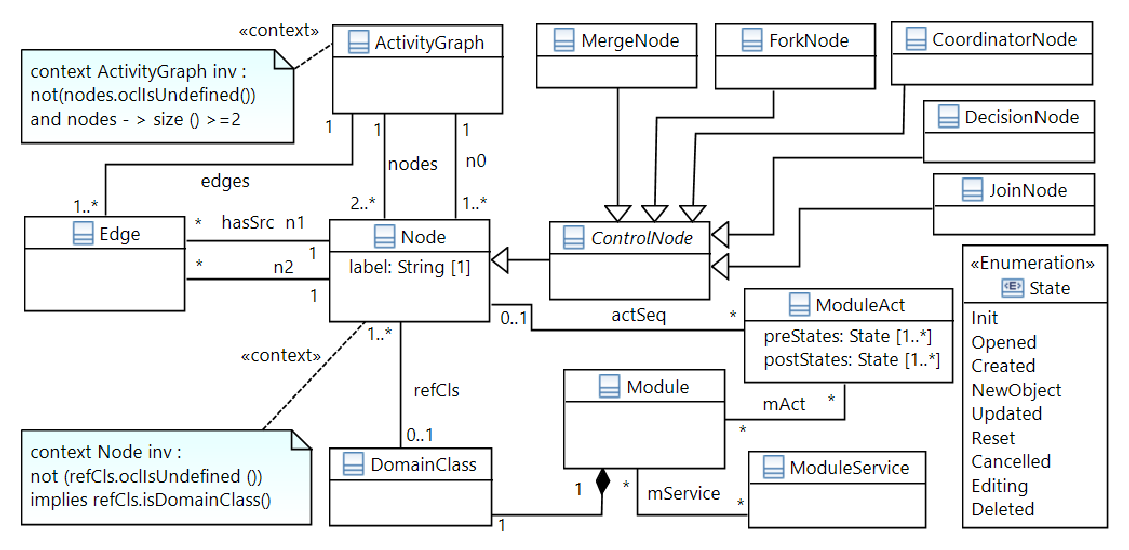
\includegraphics[scale=0.63]{agl-asm}
	\end{center}
\vspace{-0.6cm}
	\caption{A simplified metamodel for AGL's abstract syntax.} %
	\label{fig:agl-abstractSyntax}
	\vspace{-0.2cm}
\end{figure*}

Figure~\ref{fig:agl-abstractSyntax} depicts a simplified metamodel for \agl's abstract syntax. %
%~\ref{apex:agl-rules}. 
%
%To unify the notation with the unified model, in the text we will express the concepts of this model using the equivalent \dcsl's terms (see Section~\ref{sect:bg-dcsl}). This is possible because the model only contains elements (class, attribute, one-one and one-many associations and generalization) that are expressible by \dcsl.
%
Specifically, the \agl~metamodel includes the meta-concepts taken from the UML metamodel for the activity graph model: \clazz{ActivityGraph}, \clazz{Node}, \clazz{ControlNode}, and \clazz{Edge}. We define several restrictions on \clazz{Node} to form AGL's domain of activity graphs, that should be narrower (as a subset of) UML's domain of activity graphs.

Meta-concept \clazz{Node} represents activity nodes and has four properties. Attribute \attribn{label} represents the node label. 
Property \attribn{out} is derived from the association \clzassoc{hasSrc}{Edge}{Node}, which records the outgoing edges from a \clazz{Node}. The next two properties specify the referenced module that is referenced by this node. Specifically, property \attribn{refCls} references the domain class of the \textit{ref} module. 
%We call this class the \textit{ref} domain class. Here, we assume \clazztpl{Class}{\clazz{DomainClass}} represents the Domain Class concept of \dcsl~(see Section~\ref{sect:bg-dcsl}).
%
Property \attribn{serviceCls} specifies the actual \clazz{ModuleService} class of the module. It is through a module service object of \attribn{serviceCls} that the current \clazz{Node} is able to perform the \clazz{ModuleAct}s specified by the property \attribn{actSeq}. This property corresponds to the target role of the association from \clazz{Node} to \clazz{ModuleAct}. Meta-concept~\clazz{CoordinatorNode} is used to represent a task group. It does not pass its data out to the outgoing edges. Instead, it passes the original input data out. The coordinator's UI serves as the container of those of the member tasks, so that the user can have a whole picture of the group. The member tasks themselves interact with each other to perform the group's logic. An example for this meta-concept is shown in Section~\ref{sect:caseStudyToolSupport}.

Meta-concept \clazz{ModuleAct} represents SAA-typed module actions as defined in Definition~\ref{def:saa}. Note that we use an enumeration called \clazz{ActName} and an enumeration called \clazz{State} to represent the action names and the union of pre-states and post-states (\resp). \clazz{State}, in particular, represents both normal states and concurrent states (see Section~\ref{sect:arch-atomic-action}).

We need to provide well-formedness (WFRs) rules for the metamodel to obtain valid \agl models. They might be divided into two parts: (1) WFRs from UML metamodel for valid activity graphs; (2)~WFRs to ensure \agl models obtained as a composition of available domain behavior patterns. Figure~\ref{fig:agl-abstractSyntax} just shows two WFRs. For a full specification of the well-formedness OCL rules for this metamodel, we would refer the reader to the technical report~\cite{dang2023aglTechReport} for this paper.

%
%\begin{description}
%%\subsubsection*{\clazz{ModuleAct}}\label{sect:agl-cm-moduleact}
%\item[\clazz{ModuleAct}.] This represents SAA-typed module actions as defined in Definition~\ref{def:saa}. Field \attribn{actName} realizes the action name. The three fields \attribn{preStates}, \attribn{postStates}, and \attribn{output} realize three similarly-named attributes of the action.
%%
%The two fields \attrib{ModuleAct}{fieldNames} and  \attribn{fieldVals}  together realize the attribute \membern{fieldValSet} of the action, as follows: Each pair $ (f,v) $ in \membern{fieldValSet} is constructed by taking $f$ from \attribn{fieldNames} and $v$ from the corresponding element of \attribn{fieldVals}.
%%
%%\subsubsection*{\clazz{ActivityGraph}}\label{sect:agl-cm-activity-graph}
%\item[\clazz{ActivityGraph}.] This represents activity graphs and has three properties: \attribn{nodes}, \attribn{edges}, and \attribn{n0}. The first two ones correspond to the target role name of the associations to \clazz{Node} and \clazz{Edge} (\resp). The property \attribn{n0} realizes a subset of nodes that are the start nodes of the graph. The starting nodes are the ones that are invoked first when the graph is executed.
%%
%%\subsubsection*{\clazz{Node}} \label{sect:agl-cm-ctrl-node}
%\item[\clazz{Node}.] This represents activity nodes and has four properties. Attribute \attribn{label} realizes the node label. 
%%Field \attribn{out} is derived from the association \clzassoc{hasSrc}{Edge}{Node}, which records the outgoing edges from a \clazz{Node}. 
%The next two fields specify the \textbf{referenced (abbrv. \textit{ref}) software module}, i.e., the module that is referenced by this node. Specifically, field \attribn{refCls} (typed \clazztpl{Class}{\clazz{DomainClass}}) specifies the domain class of the \textit{ref} module. We call this class the \textit{ref} domain class. Here, we assume \clazztpl{Class}{\clazz{DomainClass}} represents the Domain Class concept of \dcsl~(see Section~\ref{sect:bg-dcsl}).
%%
%Field \attribn{serviceCls} (typed \clazztpl{Class}{\clazz{ModuleService}}) specifies the actual \clazz{ModuleService} class of the \textit{ref} software module. It is through a module service object of \attribn{serviceCls} that the current \clazz{Node} is able to perform the \clazz{ModuleAct}s specified by the field \attribn{actSeq}. This field is an associative field that realizes the association from \clazz{Node} to \clazz{ModuleAct}.
%%
%%\subsubsection*{\clazz{ControlNode}} \label{sect:agl-control-node}
%\item[\clazz{ControlNode}.] This is an abstract sub-type of \clazz{Node} that represents the control nodes of the activity graph. This class is used to specify the behavior of control nodes and to capture the state of its execution. We specialize class \clazz{ControlNode} into the four sub-types: \clazz{DecisionNode}, \clazz{ForkNode}, \clazz{JoinNode}, and \clazz{MergeNode}. 
%In particular, class \clazz{DecisionNode} references an interface named \clazz{Decision}, which provides a method (named \membern{evaluate}) for evaluating the decision logic. Similarly, class \clazz{JoinNode} references interface \clazz{Join}, which has a method (named \membern{transf}) for transforming the input tokens into output ones (if needed).
%Further, class \clazz{JoinNode} has a field named \attribn{pre}, which is a derived field that realizes the source \clazz{Node}s of the activity edges connecting to a \clazz{JoinNode}.
%%
%Actual implementations of the interface \clazz{Decision} (\clazz{Join}) are provided in the corresponding decision (join) classes in the unified model.
%%
%%\subsubsection*{\clazz{Edge}} \label{sect:agl-cm-edge}
%\item[\clazz{Edge}.] This represents activity edges. It has two associative fields \attribn{n1} and \attribn{n2}, which realize the two associations to \clazz{Node}. Field \attribn{n1} captures the source node, while field \attribn{n2} captures the target one. Intuitively, there is a correspondence between an \clazz{Edge} and an association between the two domain classes that are referenced by the source and target nodes of the edge.
%\end{description}

%%%%%%%%%%%%%%%%%%%%%%%%%%%%%%%%%%%%%%%%%%%%%%%%%%%%%%%%%%%
%\subsection{Concrete Syntax Model~(CSM)} 
%\label{sect:agl-asm}
%%%%%%%%%%%%%%%%%%%%%%%%%%%%%%%%%%%%%%%%%%%%%%%%%%%%%%%%%%%

%%%%%%%%%%%%%%%%%%%%%%%%%%%%%%%%%%%%%%%%%%%%%%%%%%%%%%%%%%%
\subsection{Annotation-Based Textual Concrete Syntax} 
\label{subsect:agl-textual}
%%%%%%%%%%%%%%%%%%%%%%%%%%%%%%%%%%%%%%%%%%%%%%%%%%%%%%%%%%%

We aim to define an annotation-based textual concrete syntax for \agl. To obtain this goal, we define a metamodel for the concrete syntax~(CSM) of the \agl~by a transformation from the abstract syntax ASM. Figure~\ref{fig:agl-txtSyntax} shows the CSM that takes the annotation-based form, suitable for being embedded into a host OOPL. Furthermore, we will strive for a compact CSM that uses a small set of annotations. From a practical standpoint, such a model is desirable since it will result in a compact concrete syntax, which requires less effort from the language used to construct a unified domain model.

\begin{figure*}[ht]
	\begin{center}
		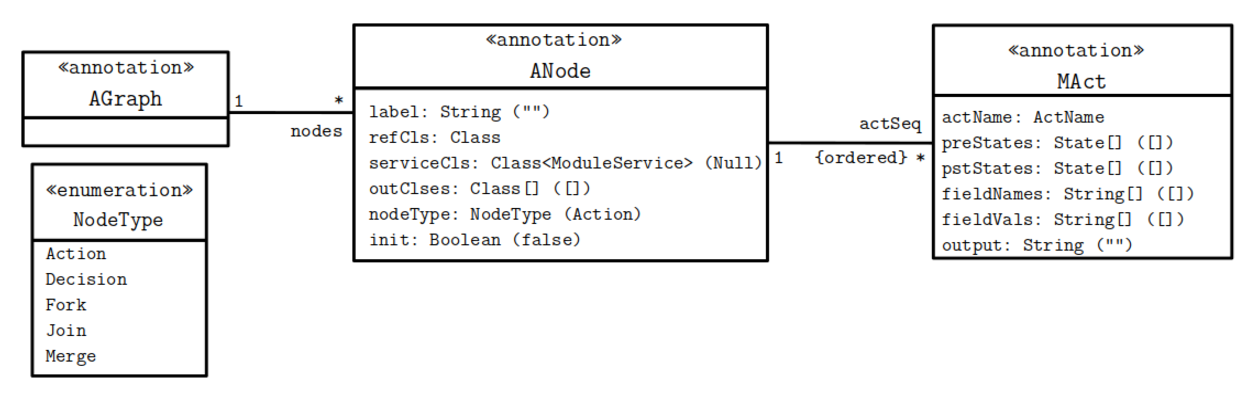
\includegraphics[scale=0.7]{agl-txtSyntax}
	\end{center}
	\vspace{-0.5cm}
	\caption{Illustration for AGL's annotation-based textual concrete syntax, realized in Java.} %
	\label{fig:agl-txtSyntax}
\end{figure*}

To realize the transformation, we proceed in two steps. First, we transform ASM into the meta-model CSM$_T$ that is compact and suitable for annotation-based representation. CSM$_T$ consists of three meta-concepts: activity graph (\clazz{AGraph}), activity node (\clazz{ANode}), and module action (\clazz{MAct}). Second, we transform CSM$_T$ into the actual annotation-based CSM that is ``embedded'' into OOPL. This transformation is required because although CSM$_T$ is suitable for OOPL's representation, it is still not yet natively in that form. This CSM is constructed from the following three OOPL meta-concepts that is discussed in Section~\ref{sect:bg-dcsl}: \clazz{class}, \clazz{annotation}, and \clazz{property}. Because CSM is embedded directly into OOPL, its structure helps define the core structure of a CSM model of the \agl's textual syntax. Adapting the concrete syntax meta-modeling approach~\cite{kleppe_software_2008} to \agl, we argue that its CSM will contain, in addition to the above core, meta-concepts that help describe the structure of the BNF grammar rules. The textual syntaxes of Java and C\# are both described using this grammar. For a detailed explanation of the transformation ASM $\rightarrow$ CSM$_T$, we would refer the reader to Appendix B of the technical report~\cite{dang2023aglTechReport} for this paper. 
%Theorem~\ref{theo:csmt-csm} as shown in \ref{apex:agl-asm2csmt} ensures that \agl's CSM has the same information capacity as CSM$_T$ through the transformation.

\noindent \textbf{Example.} The bottom-right of Figure~\ref{fig:decisional-form} depicts the configured unified model of \courseman's enrolment management activity. In this figure, the entire \agl~ specification is defined by an \clazz{AGraph} element, which is written within a note box
attached to the activity class \clazz{EnrolmentMgmt} of the unified model. For exposition purposes in this paper, we will textually write an \agl~specification using the structured note box notation of \dcsl, as explained in Section~\ref{sect:bg-dcsl}. 

%%%%%%%%%%%%%%%%%%%%%%%%%%%%%%%%%%%%%%%%%%%%%%%%%%%%%%%%%%%%%%%%
%\subsubsection{CSM$_T$: A Compact and Annotation-Friendly Model}
%%\label{sect:agl-csmt}
%%%%%%%%%%%%%%%%%%%%%%%%%%%%%%%%%%%%%%%%%%%%%%%%%%%%%%%%%%%%%%%%
%%
%Figure~\ref{fig:agl-csm}(A) shows an annotation-friendly version of the ASM, called CM$_T$, which consists of three meta-concepts: activity graph (\clazz{AGraph}), activity node (\clazz{ANode}), and module action (\clazz{MAct}). To ease discussion later about the annotation-based CSM, we add to the figure the default value notation of the optional domain field (i.e., field with \attrib{DAttr}{optional} = \code{true}). The default value is written within a pair of brackets that immediately follow the field's data type.
%%
%We briefly describe below the three meta-concepts of CSM$_T$. The precise meaning of these meta-concepts will be explained through a transformation that we define in the next section. 
%
%\begin{figure*}[ht]
%	\begin{center}
%		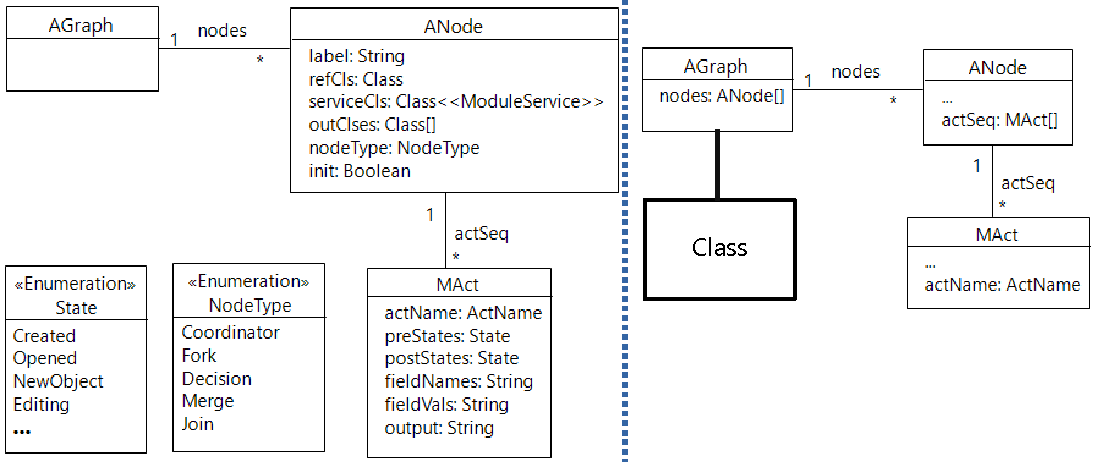
\includegraphics[scale=0.15]{agl-cmt-csm}
%	\end{center}
%	\caption{(A) CSM$_T$: a compact and annotation-friendly model, (B) The concrete syntax model (CSM) of AGL} %
%	\label{fig:agl-csm}
%\end{figure*}
%
%% TODO:   + validation function
%Note that due to the restrictions on the data type of annotation property, fields of certain meta-concepts in the ASM are not translated directly to fields in the CSM$_T$. In these cases, however, we compensate for the information loss by adding OCL constraints to the corresponding meta-concepts of the CSM$_T$. These constraints are realized by validation functions that are performed on these meta-concepts, when they are translated into the annotation form.
%%
%\begin{description}
%%\subsubsection*{\clazz{MAct}} %\label{sect:agl-csmt-mact}
%\item[\clazz{MAct}.] \clazz{MAct} realizes \clazz{ModuleAct} using only the data types that are supported by annotation. Specifically, the data types of \attrib{MAct}{preStates} and \attribn{pstStates} (the latter is short for \attribn{postStates}) are arrays of \clazz{State}. The default values of these fields are an empty array (\code{[]}), which do not mean that they are not specified. An empty array in this case means that it takes the default state value of the action as specified in Table~\ref{tab:core-atomic-actions} of Section~\ref{sect:arch-atomic-action}.
%The following additional OCL constraints help ensure that the two fields contain unique values, which are required to match the \clazz{Set} data type of the two corresponding fields of \clazz{ModuleAct}.
%% TODO: + MAct
%% + OCL constraint on preStates, pstStates
%\begin{lstrule}
%-- MAct.preStates and pstStates (if specified) contain unique values
%context Node inv:
%  not(preStates.oclIsUndefined()) implies preStates->asSet() = preStates and 
%  not(pstStates.oclIsUndefined()) implies pstStates->asSet() = pstStates
%\end{lstrule}
%
%As for the two fields \attrib{MAct}{fieldNames} and \attribn{fieldVals}, they also take an array type. This is equivalent to the \clazz{Seq} data type of the two corresponding fields of \clazz{ModuleAct}. Note that \attribn{fieldVals} is typed \clazz{String[]}, i.e., the value objects, if specified, need to be written explicitly as a string. Fortunately, this is not at all troublesome, because \attribn{fieldVals} is only required if the value objects are specified by the user. In many cases, however, the values come from another action or an external system. In these cases, \clazz{fieldVals} need not be specified and can take the default value of an empty array.
%
%Last but not least, field \attrib{MAct}{output} is typed \clazz{String} and has the default value of an empty string (\strq{}). This field is added only for completeness. It always takes the default value, because the output value of a module action is never specified by the user. It is generated from within the system.
%%
%%\subsubsection*{\clazz{ANode}} \label{sect:agl-cmt-anode}
%\item[\clazz{ANode}.] Class \clazz{ANode} both represents \clazz{Node} and \clazz{Edge} and merges the entire \clazz{ControlNode} type hierarchy. To achieve the former, we add to \clazz{ANode} a new field, named \membern{outClses}, that captures the \textit{ref} domain classes of the target nodes of the outgoing edges of a node. To achieve the latter, we add to \clazz{ANode} a field named \attribn{nodeType}, whose data type is the enumeration \clazz{NodeType}. This enumeration specifies all the pre-defined node types, including action and control types.
%
%%TODO: + ANode
%% + add extra OCL constraints for the above
%\begin{lstrule}
%-- ANode.refCls and ANode.outClses (if specified) are domain classes
%context Node inv:
%  not(refCls.oclIsUndefined()) implies refCls.isDomainClass() and 
%  not(outClses.oclIsUndefined()) implies outClses->forAll(isDomainClass())
%\end{lstrule}
%
%Note that we cannot explicitly define the data types of \attrib{ANode}{refCls} and \attribn{outClses} as parameterized types of \clazz{DomainClass}, because this class only exists in the ASM and not in the actual annotation-based model. We compensate for this information loss in the two data types by two OCL constraints on \clazz{ANode} for the two fields. Both constraints (listed immediately above) make use of a boolean function named \func{isDomainClass}. This function, which is defined as part of the ASM's library rules in Appendix A.6 of the technical report\footnote{\url{https://tinyurl.com/AGLTechnical}} of this paper, %~\ref{apex:agl-Class}, 
%is invoked on a class to check if it is attached to a \clazz{DClass} element. 
%%
%%\subsubsection*{\clazz{AGraph}} \label{sect:agl-cmt-agraph}
%\item[\clazz{AGraph}.] Class \clazz{AGraph} is simplified from \clazz{ActivityGraph} by having just one associative field for \clazz{ANode}. To further simplify this graph and ease its configuration, we replace the field \attrib{ActivityGraph}{n0} by a new boolean-typed field \attrib{ANode}{init}. We reconstruct \attrib{ActivityGraph}{n0} from all \clazz{ANode}s that have \attribn{init} = \code{true}.
%\end{description}


%%%%%%%%%%%%%%%%%%%%%%%%%%%%%%%%%%%%%%%%%%%%%%%%
%\subsubsection{The Annotation-Based CSM}
%\label{sect:agl-csm}
%%%%%%%%%%%%%%%%%%%%%%%%%%%%%%%%%%%%%%%%%%%%%%%%
%
%Although CSM$_T$ is suitable for OOPL's representation, it is still not yet natively in that form. Our next step, therefore, is to transform it into a CSM that is ``embedded'' into OOPL. This CSM is constructed from the following three OOPL meta-concepts that were discussed in Section~\ref{sect:bg-dcsl}: class, annotation, and property.
%
%%\begin{figure*}[ht]
%%	\begin{center}
%%		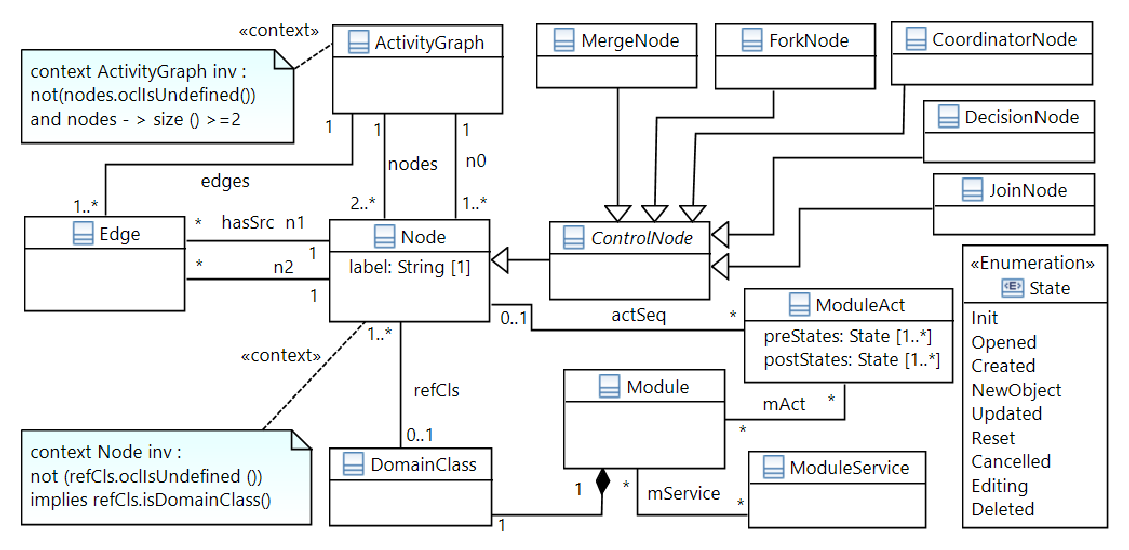
\includegraphics[scale=0.4]{agl-asm}
%%	\end{center}
%%	\caption{The concrete syntax model (CSM) of \agl.} %
%%	\label{fig:agl-csm}
%%\end{figure*}
%
%Figure~\ref{fig:agl-csm}(B) shows the metamodel in the form of a UML class diagram for ASM. In this, the three meta-classes in CSM$_T$ are transformed into three annotations of the same name. The annotations are represented in the figure as 2-part grey-colored boxes, the association lines as grey lines. Each domain field is transformed into an annotation property. The non-associative domain fields are transformed directly into properties and so, to ease reading, we use `\dots' to represent these properties. We only highlight in the figure two properties of the two associative fields \attrib{AGraph}{nodes} and \attrib{ANode}{actSeq}. 
%
%A key difference between CSM and CSM$_T$ is the attachment of \clazz{AGraph} to \clazz{Class}. This is represented in Figure~\ref{fig:agl-csm}(B) by a solid line connecting the two corresponding class boxes. An \clazz{AGraph} attachment defines an AGC because it describes the instantiation of an \clazz{AGraph} object together with the associated \clazz{ANode}s and \clazz{MAct} objects.
%
%Adding the \clazz{AGraph} attachment to our definition of activity class (see Definition~\ref{def:unified-class-model}) helps form a bridge between \agl~and the unified model. More specifically, in the overall context of our method, we call any class that has an \clazz{AGraph} attachment an \textit{activity class}.
%Further, to ease discussion we will use the term \textbf{configured unified model} to refer to a unified model whose activity class is attached with an \clazz{AGraph}. 
%%
%\subsubsection*{Discussion} \label{sect:agl-discussion} %
%In the current syntax, the AGC is sensibly attached to the activity class, because this class serves as the pivot for the activity graph definition.
%%
%An alternative annotation-based syntax would be to not define the \clazz{ANode}s as a property of \clazz{AGraph} (i.e., to remove property \attrib{AGraph}{nodes}), but to distribute them such that they are attached to the domain classes that they reference (via the property \attrib{ANode}{refCls}). 
%
%However, this syntax has several limitations. First, we need extra properties in order to keep track of which \clazz{ANode}s belong to which \clazz{AGraph}. For example, we need two new properties \attrib{AGraph}{id} and \attrib{ANode}{graph}, the values of which in the same \clazz{AGraph} are equal. 
%Second, it is more difficult to read, understand, and validate the AGC. This is because the AGC is not in one place but is scattered around in different parts of the domain model.
%Third, we would unnecessarily complicate the component classes with \clazz{ANode} specifications, which in turn would hinder their use and understandability. These classes should only be concerned with the domain logic, not the mechanics of the activity graph that executes them.
%
%%%%%%%%%%%%%%%%%%%%%%%%%%%%%%%%%%%%%%%%%%%%%%%%%%%%%%%%%%%%%%%%
%\subsection{Annotation-Based Textual Concrete Syntax} 
%\label{sect:agl-csSyntax}
%%%%%%%%%%%%%%%%%%%%%%%%%%%%%%%%%%%%%%%%%%%%%%%%%%%%%%%%%%%%%%%%

%Because CSM is embedded directly into OOPL, its structure helps define the core structure of a CSM model of the \agl's textual syntax. Adapting the concrete syntax meta-modeling approach~\cite{kleppe_software_2008} to \agl, we argue that its CSM will contain, in addition to the above core, meta-concepts that help describe the structure of the BNF grammar rules. The textual syntaxes of Java and C\# are both described using this grammar.
%%
%For exposition purposes in this paper, we will textually write an AGC using the structured note box notation of \dcsl~(explained in Section~\ref{sect:bg-dcsl}). 
%
%The following example will help to illustrate.

%\begin{figure}[ht]
%	\begin{center}
%		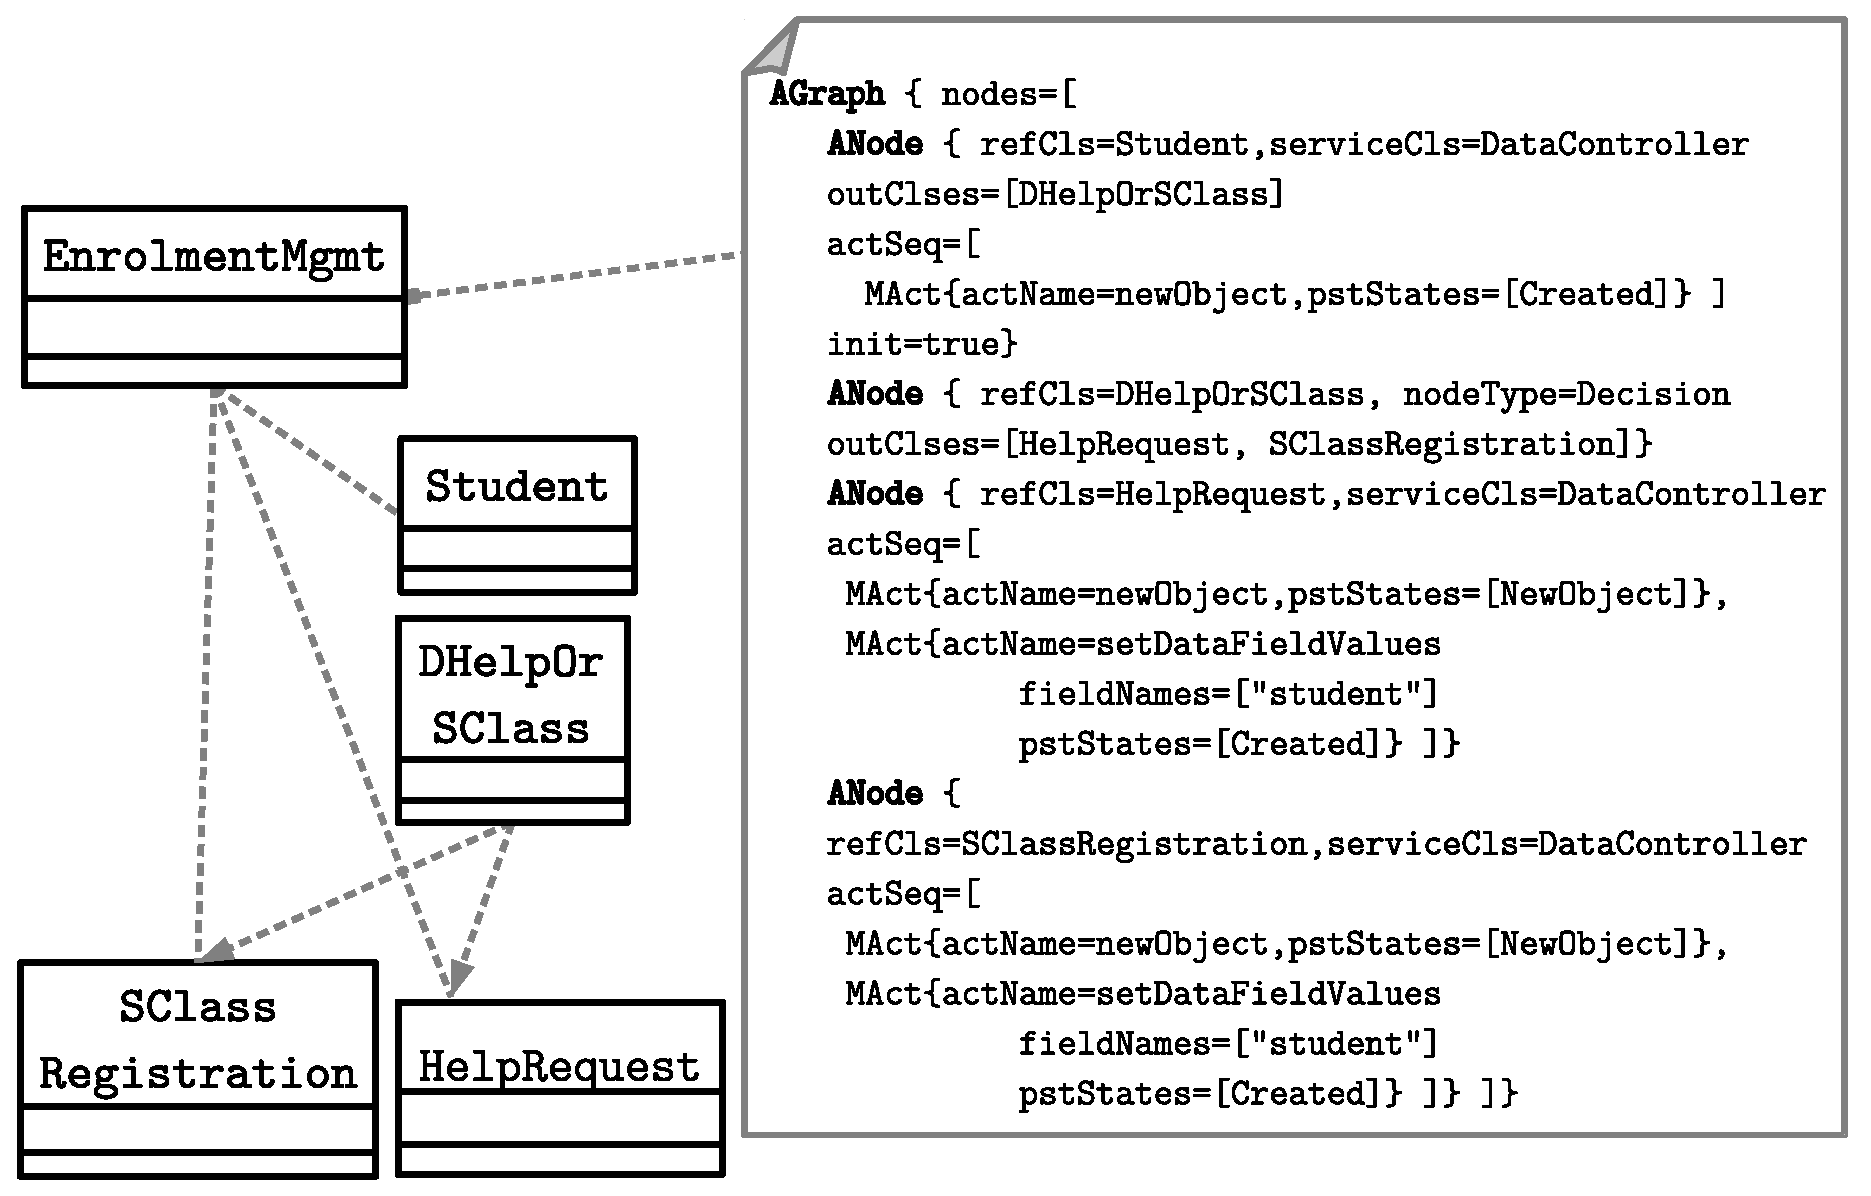
\includegraphics[scale=0.35]{agc-enrolmentmgmt}
%	\end{center}
%	\caption{Configured unified model of the enrolment management activity: (LHS) the unified model, (RHS) the AGC written in the annotation-based concrete syntax.} %
%	\label{fig:agc-enrolmentmgmt}
%\end{figure}

%Figure~\ref{fig:agc-enrolmentmgmt} depicts the configured unified model of the enrolment management activity shown in  Figure~\ref{fig:activity-graph-example}. As shown in Figure~\ref{fig:agc-enrolmentmgmt}, the entire AGC is defined by an \clazz{AGraph} element, which is written within a note box attached to the activity class \clazz{EnrolmentMgmt} of the unified model.
%
%As can be seen from the figure, the \clazz{AGraph} element is configured with its property \attribn{nodes} being set to an array of four \clazz{ANode}s. These \clazz{ANode}s configure the four \clazz{Node} objects listed earlier in Table~\ref{tab:activity-graph-example}, and additionally for each of them the component class(es) that will become the referenced domain classes of the target nodes of the outgoing edges (if any). These component class(es) are specified by property \attrib{ANode}{outClses}. For example, the first \clazz{ANode} configures the state of the node \objid{1}{Node}. Property \attribn{outClses} of this \clazz{ANode} is set to the array [\clazz{DHelpOrSClass}], which states that \objid{1}{Node} has an outgoing edge whose target node is the node whose \textit{ref} domain class is \clazz{DHelpOrSClass}. According to Table~\ref{tab:activity-graph-example} this is node \objid{2}{Node}, and the outgoing edge is \objid{1}{Edge}.